\documentclass[10pt, conference, compsocconf]{IEEEtran}

%\usepackage[numbers, sort, compress]{natbib}
\usepackage{graphicx}
\usepackage{amsmath}
\usepackage{amssymb}
\usepackage{color}
\usepackage{ifpdf}
%\usepackage{mdwlist}

%\usepackage{dcolumn}
\usepackage{float}
\usepackage[utf8]{inputenc}
\usepackage{multirow}
\usepackage{rotating}
\usepackage{subfigure}

\usepackage{moresize}
%\usepackage{setspace}

%\usepackage[numbers, sort, compress]{natbib}
%\usepackage{latex8}
%\usepackage{float}
%\usepackage{times}    
\usepackage{url}
\usepackage{booktabs}
\usepackage{listings}   
\usepackage{paralist}    
\usepackage{wrapfig}    
%\usepackage[footnotesize,it]{caption}
\usepackage{multirow}
\usepackage{ifpdf}
%\usepackage{srcltx}
%\usepackage{subfigure}
\usepackage{xspace}
\usepackage{keyval}  
\usepackage{color}
\usepackage{listings}
\usepackage{comment}

%\usepackage{draftwatermark}
%\SetWatermarkLightness{0.8}
%\SetWatermarkText{Draft}
%\SetWatermarkVerCenter{13cm}
%\SetWatermarkHorCenter{10cm}
%\SetWatermarkScale{1} 

\definecolor{listinggray}{gray}{0.95}
\definecolor{darkgray}{gray}{0.7}
\definecolor{commentgreen}{rgb}{0, 0.4, 0}
\definecolor{darkblue}{rgb}{0, 0, 0.4}
\definecolor{middleblue}{rgb}{0, 0, 0.7}
\definecolor{darkred}{rgb}{0.4, 0, 0}
\definecolor{brown}{rgb}{0.5, 0.5, 0}
\definecolor{dkgreen}{rgb}{0,0.5,0}
\definecolor{orange}{rgb}{1,.5,0}
\definecolor{dandelion}{cmyk}{0,0.29,0.84,0}

\usepackage[normalem]{ulem}
\makeatletter
\def\cyanuwave{\bgroup \markoverwith{\lower3.5\p@\hbox{\sixly \textcolor{cyan}{\char58}}}\ULon}
\def\reduwave{\bgroup \markoverwith{\lower3.5\p@\hbox{\sixly \textcolor{red}{\char58}}}\ULon}
\def\blueuwave{\bgroup \markoverwith{\lower3.5\p@\hbox{\sixly \textcolor{blue}{\char58}}}\ULon}
\font\sixly=lasy6 % does not re-load if already loaded, so no memory problem.
\makeatother

\let\labelindent\relax
\usepackage{enumitem}

%\usepackage{xcolor}
\newif\ifdraft
\drafttrue
\ifdraft
 \newcommand{\N}[1]{\textbf{NOTE: #1}\xspace}
 \newcommand{\jhanote}[1]{ {\textcolor{red} { ***SJ: #1 }}}
 \newcommand{\katznote}[1]{ {\textcolor{blue} { ***DSK: #1 }}}
 \newcommand{\mtnote}[1]{ {\textcolor{orange} { ***MT: #1 }}}
 \newcommand{\jonnote}[1]{ {\textcolor{dkgreen} { ***JW: #1 }}}
 \newcommand{\aanote}[1]{ {\textcolor{dkgreen} { ***AA: #1 }}}
 \newcommand{\note}[1]{ {\textcolor{brown} { *** #1 }}}
 \newcommand{\sarp}[1]{{\color{red}\textit{sarp: {#1}}}}
\else
 \newcommand{\N}[1]{}
 \newcommand{\jhanote}[1]{}
 \newcommand{\katznote}[1]{}
 \newcommand{\mtnote}[1]{}
 \newcommand{\jonnote}[1]{}
 \newcommand{\sarp}[1]{}
 \newcommand{\note}[1]{}
\fi

\newif\ifdraft
%\drafttrue
\ifdraft
\newcommand{\terminology}[1]{ {\textcolor{red} {(Terminology used: \textbf{#1}) }}}
\newcommand{\owave}[1]{ {\cyanuwave{#1}}}
\newcommand{\jwave}[1]{ {\reduwave{#1}}}
\newcommand{\alwave}[1]{ {\blueuwave{#1}}}
\newcommand{\alnote}[1]{ {\textcolor{blue} { ***andreL: #1 }}}
\newcommand{\amnote}[1]{ {\textcolor{blue} { ***andreM: #1 }}}
\newcommand{\smnote}[1]{ {\textcolor{brown} { ***sharath: #1 }}}
\newcommand{\pmnote}[1]{ {\textcolor{brown} { ***Pradeep: #1 }}}
\newcommand{\msnote}[1]{ {\textcolor{cyan} { ***mark: #1 }}}
\newcommand{\mrnote}[1]{ {\textcolor{purple} { ***melissa: #1 }}}
%\newcommand{\mtnote}[1]{ {\textcolor{orange} { ***matteo: #1 }}}
\else
\newcommand{\onote}[1]{}
\newcommand{\terminology}[1]{}
\newcommand{\owave}[1]{#1}
\newcommand{\jwave}[1]{#1}
\newcommand{\alnote}[1]{}
\newcommand{\amnote}[1]{}
\newcommand{\athotanote}[1]{}
\newcommand{\smnote}[1]{}
\newcommand{\pmnote}[1]{}
\newcommand{\msnote}[1]{}
\newcommand{\mrnote}[1]{}
\newcommand{\aznote}[1]{}
%\newcommand{\mtnote}[1]{}
\fi

\newcommand{\cloud}{cloud\xspace}
\newcommand{\clouds}{clouds\xspace}
\newcommand{\pilot}{Pilot\xspace}
\newcommand{\pilots}{Pilots\xspace}
\newcommand{\pilotjob}{Pilot-Job\xspace}
\newcommand{\pilotjobs}{Pilot-Jobs\xspace}
\newcommand{\pilotcompute}{Pilot-Compute\xspace}
\newcommand{\pilotcomputedescription}{Pilot-Compute Description\xspace}
\newcommand{\pilotdescription}{Pilot-Description\xspace}
\newcommand{\pilotcomputes}{Pilot-Computes\xspace}
\newcommand{\pilotdata}{Pilot-Data\xspace}
\newcommand{\pilotdatadescription}{Pilot-Data Description\xspace}
\newcommand{\pilotdataservice}{Pilot-Data Service\xspace}
\newcommand{\pilotcomputeservice}{Pilot-Compute Service\xspace}
\newcommand{\computedataservice}{Compute-Data Service\xspace}
\newcommand{\computeunitdescription}{Compute-Unit Description\xspace}
\newcommand{\dataunitdescription}{Data-Unit Description\xspace}
\newcommand{\pilotmapreduce}{PilotMapReduce\xspace}
\newcommand{\mrmg}{MR-Manager\xspace}
\newcommand{\pstar}{P*\xspace}
\newcommand{\pd}{PD\xspace}
\newcommand{\pc}{PC\xspace}
\newcommand{\pcs}{PCs\xspace}
\newcommand{\pj}{PJ\xspace}
\newcommand{\pjs}{PJs\xspace}
\newcommand{\pds}{Pilot Data Service\xspace}
\newcommand{\computeunit}{Compute-Unit\xspace}
\newcommand{\computeunits}{Compute-Units\xspace}
\newcommand{\dataunit}{Data-Unit\xspace}
\newcommand{\dataunits}{Data-Units\xspace}
\newcommand{\du}{DU\xspace}
\newcommand{\dus}{DUs\xspace}
\newcommand{\dud}{DUD\xspace}
\newcommand{\cu}{CU\xspace}
\newcommand{\cus}{CUs\xspace}
\newcommand{\cud}{CUD\xspace}
\newcommand{\su}{SU\xspace}
\newcommand{\sus}{SUs\xspace}
\newcommand{\schedulableunit}{Schedulable Unit\xspace}
\newcommand{\schedulableunits}{Schedulable Units\xspace}
\newcommand{\cc}{c\&c\xspace}
\newcommand{\CC}{C\&C\xspace}
\newcommand{\up}{\vspace*{-1em}}
\newcommand{\upp}{\vspace*{-0.5em}}
\newcommand{\numrep}{8 }
\newcommand{\samplenum}{4 }
\newcommand{\tmax}{$T_{max}$ }
\newcommand{\tc}{$T_{C}$ }
\newcommand{\tcnsp}{$T_{C}$}
\newcommand{\bj}{BigJob\xspace}
\newcommand{\irods}{iRODS\xspace}

\newcommand{\I}[1]{\textit{#1}\xspace}
\newcommand{\B}[1]{\textbf{#1}\xspace}
\newcommand{\T}[1]{\texttt{#1}\xspace}
\newcommand{\C}[1]{\textsc{#1}\xspace}

\newcommand{\mr}[1]{\multirow{2}{*}{#1}}%
\newcommand{\mc}[2]{\multicolumn{#1}{l}{#2}}

\lstdefinestyle{myListing}{
  frame=single,
  backgroundcolor=\color{listinggray},
  %float=t,
  language=C,
  basicstyle=\ttfamily \footnotesize,
  breakautoindent=true,
  breaklines=true
  tabsize=2,
  captionpos=b,
  aboveskip=0em,
  belowskip=-2em,
  %numbers=left,
  %numberstyle=\tiny
}

\lstdefinestyle{myPythonListing}{
  frame=single,
  backgroundcolor=\color{listinggray},
  %float=t,
  language=Python,
  basicstyle=\ttfamily \scriptsize,
  breakautoindent=true,
  breaklines=true
  tabsize=2,
  captionpos=b,
  %numbers=left,
  %numberstyle=\tiny
}



%  \setlength{\parskip}{0.05ex} % 1ex plus 0.5ex minus 0.2ex}
%  \setlength{\parsep}{0pt}
%  %\setlength{\headsep}{0pt}
%  \setlength{\topskip}{0pt}
%  \setlength{\topmargin}{0pt}
%  %\setlength{\topsep}{0pt}
%  \setlength{\partopsep}{0pt}

% This is now the recommended way for checking for PDFLaTeX:


\ifpdf
\DeclareGraphicsExtensions{.pdf, .jpg, .tif}
\else
\DeclareGraphicsExtensions{.ps,  .eps, .jpg}
\fi

\tolerance=1000
\hyphenpenalty=10


\usepackage{listings}
\usepackage{comment}


% -----------------------------------------------------------------------------
% BEGIN DOCUMENT
% -----------------------------------------------------------------------------
\begin{document}

\title{PanDA and NGE Integration}


\author{
\IEEEauthorblockN{Authors Name/s per 1st Affiliation (Author)}
\IEEEauthorblockA{line 1 (of Affiliation): dept.\ name of organization\\
    line 2: name of organization, acronyms acceptable\\
    line 3: City, Country\\
    line 4: Email: name@xyz.com}
\and
\IEEEauthorblockN{Authors Name/s per 2nd Affiliation (Author)}
\IEEEauthorblockA{line 1 (of Affiliation): dept.\ name of organization\\
    line 2: name of organization, acronyms acceptable\\
    line 3: City, Country\\
    line 4: Email: name@xyz.com}
}

% make the title area
\maketitle

% ----------------------------------------------------------------------------
% ABSTRACT
% ----------------------------------------------------------------------------
\begin{abstract}
TBD\@.
\end{abstract}

\begin{IEEEkeywords}
TBD\@.
\end{IEEEkeywords}

% ----------------------------------------------------------------------------
% I - INTRODUCTION
% ----------------------------------------------------------------------------
\section{Introduction}
\label{sec:intro}


% ----------------------------------------------------------------------------
% II - RELATED WORK
% ----------------------------------------------------------------------------
\section{Related Work}
\label{sec:related}


% ----------------------------------------------------------------------------
% III - ARCHITECTURE
% ----------------------------------------------------------------------------
\section{Architecture}
\label{sec:panda_overview}

\begin{figure}
  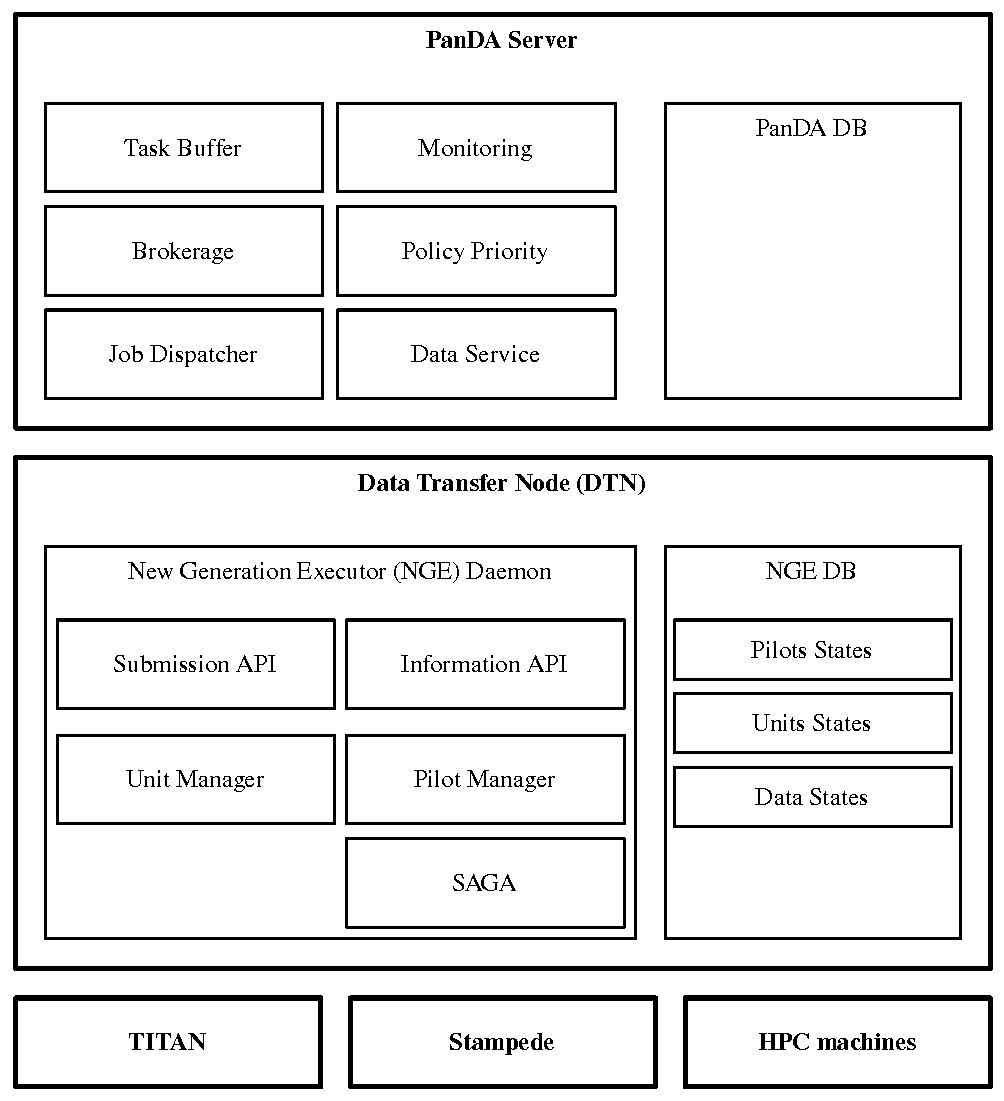
\includegraphics[width=\columnwidth]{figures/panda_nge.pdf}
  \caption{Architecture of the system integrating PanDA and NGE.}
\label{fig:atlas_workflow}
\end{figure}

\begin{itemize}

    \item General description: The next generation executer (NGE) is
    encapsulated within a daemon executed on a data transfer node (DTN) on
    Titan. The NGE daemon exposes two interfaces: one for job submission, the
    other for providing information about resources. The NGE behaves like a
    resource broker, offering information about the resources that are currently
    available and those that can become available.

    \item Interfaces: Jobs are described in terms of requirements for their
    execution and resources are described abstracting from the specifics of the
    machines on which these resources are acquired. The definition of a job
    description and of a resource description protocol are among the
    deliverables of this paper.

    \item Database: information about the resources (abstracted in terms of
    pilots), the tasks submitted for execution (abstracted in terms of compute
    units), and of the data required by each task (abstracted in terms of data
    units) are stored in the NGE DB\@. The DB is the only stateful element of the NGE architecture and, as such, will have to be fault-tolerant and redundant.

\end{itemize}

% ----------------------------------------------------------------------------
% IV - EVALUATION
% ----------------------------------------------------------------------------
\section{Evaluation}
\label{sec:evaluation}


% ----------------------------------------------------------------------------
% V - DISCUSSION
% ----------------------------------------------------------------------------
\section{Discussion}
\label{sec:discussion}


% ----------------------------------------------------------------------------
% VI - CONCLUSION
% ----------------------------------------------------------------------------
\section{Conclusion}
\label{sec:conclusion}


% ----------------------------------------------------------------------------
% ACKNOWLEDGEMENTS AND CONTRIBUTIONS
% ----------------------------------------------------------------------------
\section{Acknowledgements and Contributions}
\label{sec:ack}


% ----------------------------------------------------------------------------
% REFERENCES
% ----------------------------------------------------------------------------
\bibliographystyle{plain}
\bibliography{bibliography}

% that's all folks
\end{document}
